\begin{block}{Spatially Aggregated Temperature Extremes}
    Analyzing our ``inferred heating demand per capita'' (see Methods and Data) informs the question ``what would the aggregate demand for heating have been had historic cold snaps occurred with 2020's population?''
    \begin{framed}
        \begin{figure}
            \centering
            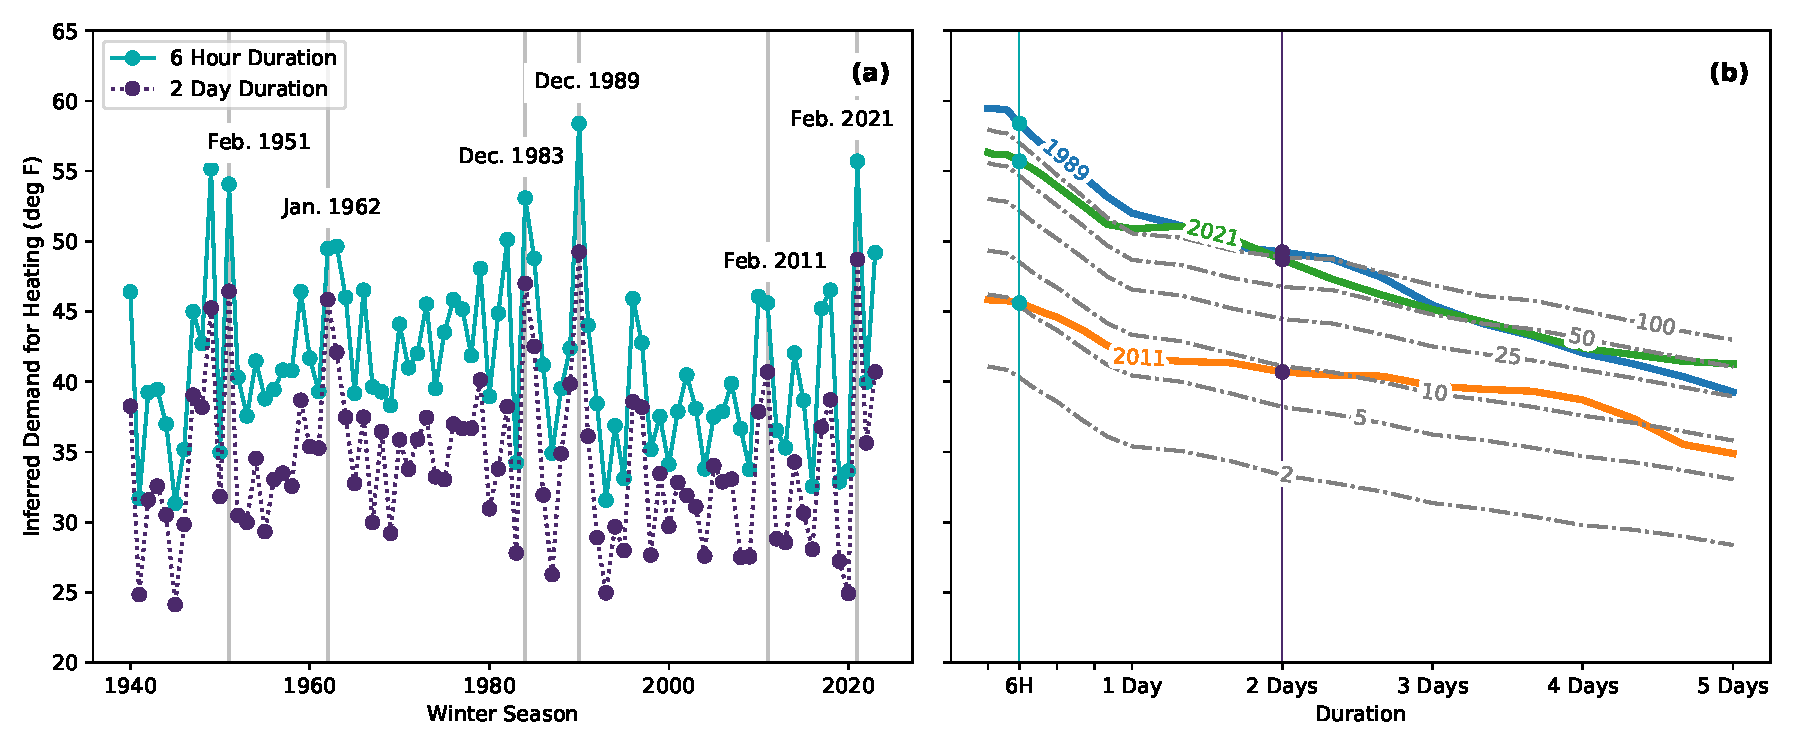
\includegraphics[width=\textwidth]{ERCOT_HDD_IDF_MLE_popweighted.pdf}\\
            \caption{
                \textbf{The inferred heating demand per capita induced by the February 2021 cold snap is not unprecedented.}
                (a): time series of annual maximum inferred heating demand per capita.
                (b): the intensity-duration-frequency intervals estimated using 1950-2020 data (i.e., not using the 2021 event), overlaid by the annual maxima from the 1989, 2011, and 2021 events.
                Gray dashed lines indicate 2, 5, 10, 25, 50, and 100 year return levels.
            }\label{fig:idf_weighted}
        \end{figure}
    \end{framed}
\end{block}